\documentclass{standalone}
\usepackage{tikz}
\usepackage{ctex,siunitx}
\usepackage{tkz-euclide}
\usepackage{amsmath}
\usetikzlibrary{patterns, calc}
\usetikzlibrary {decorations.pathmorphing, decorations.pathreplacing, decorations.shapes,decorations.markings,positioning, snakes}

\begin{document}
\small
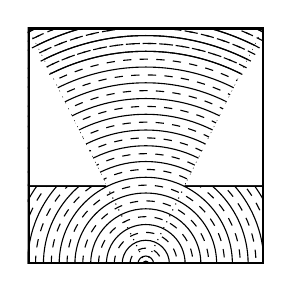
\begin{tikzpicture}[>=stealth]
  \clip (-1.5, 0) rectangle (1.5,3);
  \foreach \x in {.1,.3,...,5}
  {
      \draw (-\x,0) arc (180:0:\x);
  }
  \foreach \x in {.2,.4,...,5}
  {
  	\draw [dashed] (-\x,0) arc (180:0:\x);
  }
  
  % \fill [white](-5.1,-2) rectangle (-1.5, 6);
  % \fill [white](1.5,-2) rectangle (5.1, 6);
  \draw[ultra thick] (-1.5,1)--(-.5,1);
  \draw[ultra thick] (1.5,1)--(.5,1);
  \draw [dotted](0,0)--(-.5,1)--(-1,2)--(-1.5,3);
  \draw [dotted](0,0)--(.5,1)--(1,2)--(1.5,3);
  % \fill [white](-1.5,3) rectangle (1.5, 6);
  \fill [white](-1.5,1)--(-.5,1)--(-1.5,3)--(-1.5,1);
  \fill [white](1.5,1)--(.5,1)--(1.5,3)--(1.5,1);
  \draw [ultra thick](-1.5, 0) rectangle (1.5,3);
  \draw  [fill=black] (0,0)  circle (1pt);
  
  \draw(63:2.7) arc (63:117:2.7);
  \draw[dashed] (62.8:2.8) arc (62.8:117.2:2.8);
  \draw (62.6:2.9) arc (62.6:117.4:2.9);
  \draw[dashed] (62.4:3) arc (62.4:117.6:3);
  \draw (62.2:3.1) arc (62.2:117.8:3.1);
  \draw[dashed] (62:3.2) arc (62:118:3.2);
  \draw (61.8:3.3) arc (61.8:118.2:3.3);
  
\end{tikzpicture}
\end{document}